\documentclass{beamer}
\usetheme[faculty=fss]{fibeamer}
\usepackage[utf8]{inputenc}
\usepackage[
  main=ukrainian,english,czech, slovak ]{babel}       
  \title{\texttt{Шляхи збiльшення густини запису iнформацiї при магнiтному записi}} %% that will be typeset on the
  %\subtitle{Presentation Subtitle} %% title page.
  \author{Мнацаканов Антон}
  %% These additional packages are used within the document:
  \usepackage{ragged2e}  % `\justifying` text
  \usepackage{booktabs}  % Tables
  \usepackage{tabularx}
  \usepackage{tikz}      % Diagrams
  \usetikzlibrary{calc, shapes, backgrounds}
  \usepackage{amsmath, amssymb}
  \usepackage{url}       % `\url`s
  \usepackage{listings}  % Code listings
\frenchspacing
\begin{document}
  \shorthandoff{-}
  \frame[c]{\maketitle}


  \AtBeginSection[]{% Print an outline at the beginning of sections
    \begin{frame}<beamer>
      \frametitle{Відкриття та розвиток магнітного запису}
      \tableofcontents[currentsection]
    \end{frame}}

%--------------------------------------1
    \begin{frame}{Відкриття та розвиток магнітного запису}
      \framesubtitle{Вальдемар Поульсен}%
        \begin{figure}[h]
          \center{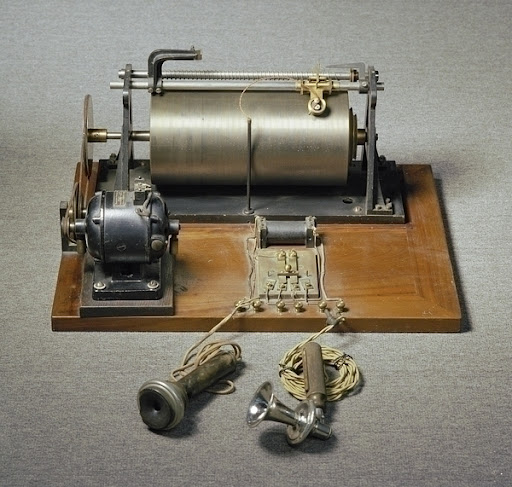
\includegraphics[width=0.6\linewidth]{2.jpg}}
          \caption{Перший апарат магнітного запису.}
          
        \end{figure}
    \end{frame}
%--------------------------------------2
    \begin{frame}[label=lists]{Структура шарів магнітної стрічки.}
 \begin{figure}[h]
    \center{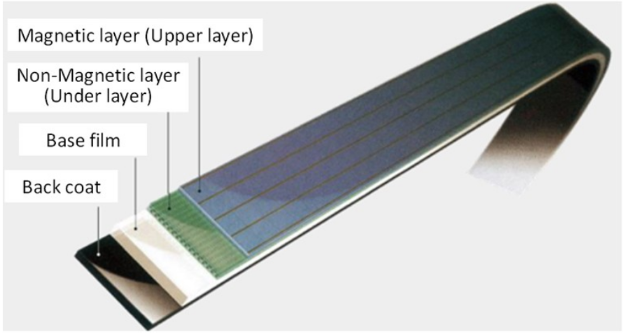
\includegraphics[width=0.8\linewidth]{1.png}}
  \end{figure}
  \begin{itemize}
    \item заднє покриття
    \item основна плівка
    \item немагнітний шар (нижній шар)
    \item немагнітний шар (верхній шар) 
  \end{itemize}
    \end{frame}
%--------------------------------------3
    \subsection{Матеріали   шарів}
    \begin{frame}[label=simmonshall]{Матеріали   шарів}
    
      \begin{block}{$Fe_2O_3$}
      \end{block}

      \begin{block}{$CrO_2$}
      \end{block}

      \begin{block}{$Fe_2O_3 + CrO_2$}
      \end{block}

      \begin{block}{$Fe$}  
      \end{block}

    \end{frame}
%--------------------------------------4
    \begin{frame}[label=proof]{Мангітні біти в дискеті}
    
    \begin{figure}[h]
    \center{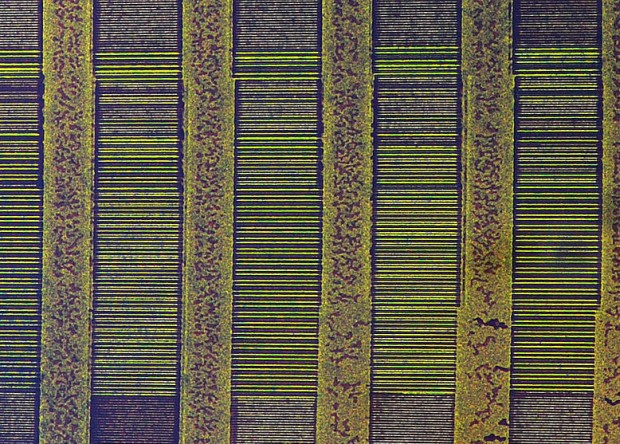
\includegraphics[width=0.9\linewidth]{5.jpg}}
    \end{figure}

    \end{frame}

%--------------------------------------5
  \begin{frame}[label=proof]{Нові розробки}
  \begin{figure}[h]
  \center{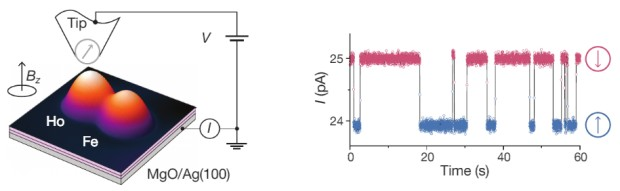
\includegraphics[width=0.99\linewidth]{6.jpg}}
  \caption{Схема експерименту (зліва). Читання станів атомів (праворуч).}
  \end{figure}
  \end{frame}

%--------------------------------------6
  \begin{frame}
  \begin{figure}[h]
  \center{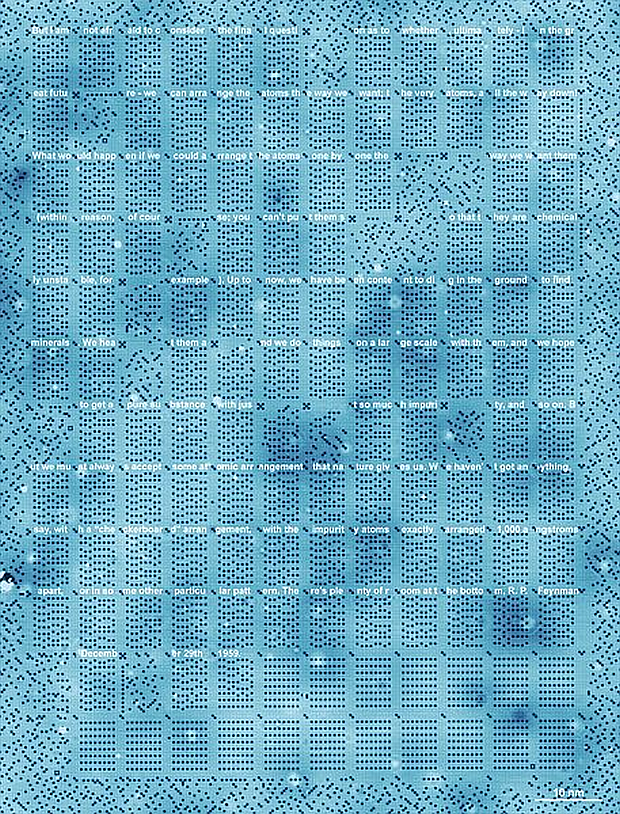
\includegraphics[width=0.6\linewidth]{9.png}}
  \label{ris9}
  \end{figure}
  \end{frame}
%--------------------------------------7
  \begin{frame} 
  \begin{figure}[h!]
  \center{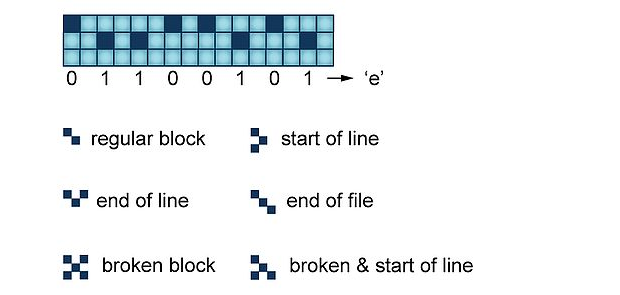
\includegraphics[width=13.5cm, height = 6cm]{10.png}}
  \caption{Принцип кодування інформації}

  \end{figure}
  \end{frame}
%--------------------------------------8
  \begin{frame}
  \begin{thebibliography}{9}
  \bibitem{lit1} Основы магнитной записи информации : учеб. пособие для студентов физического факультета / сост. : С.П. Кудрявцева. – 2017. 51 с.
  \bibitem{lit2} https://habr.com/ru/post/422851/
  \bibitem{lit3} https://nplus1.ru/news/2017/03/09/information-density-record
  \bibitem{lit4} II International Scientific Practical Conference of graduate and postgraduate students,
  lecturers «APPLIED ISSUES OF EXACT SCIENCES»
  19-20 October 2018, Armavir(http://amti.esrae.ru/pdf/2018/3(1)/197.pdf)
  \bibitem{lit5} https://compress.ru/article.aspx?id=10717part=31ext1
  \bibitem{lit6} https://compress.ru/article.aspx?id=10717
  \bibitem{lit7} https://aip.scitation.org/doi/10.1063/1.1953879
  \bibitem{lit8} \href{https://www.researchgate.net/publication/224354512_Heat_Assisted_Magnetic_Recording}{Heat Assisted Magnetic Recording}

  \end{thebibliography}
  \end{frame}

%--------------------------------------9
\begin{frame}
  \begin{center}
  \noindent{\color{blue} \rule{\linewidth}{0.7mm}}
  \Large{Дякую за увагу!}
  \noindent{\color{blue} \rule{\linewidth}{0.7mm}}
  \end{center}
\end{frame}


















\end{document}